%File: M3_submission.tex
\documentclass[letterpaper]{article}
\usepackage{xcolor}
\usepackage{flairs}
\usepackage{times}
\usepackage{helvet}
\usepackage{courier}
\usepackage{url}
\usepackage{graphicx}
\usepackage{amsmath}
\usepackage{amssymb}
\frenchspacing
\setlength{\pdfpagewidth}{8.5in}
\setlength{\pdfpageheight}{11in}
\pdfinfo{
/Title (Graph-Based Risk Mapping: Mining Road Networks to Predict Vehicular Mortality in Florida Panthers)
/Author (George Alenchery, Marcelo Amorim, Jeremy Martin)}
\setcounter{secnumdepth}{0}
\begin{document}

\title{Graph-Based Risk Mapping: Mining Road Networks to Predict Vehicular Mortality in Florida Panthers \\ \vspace{0.15em} \normalsize{CAI 6107 Fall 2026}}
% \author{George Alenchery, Marcelo Amorim, and Jeremy Martin \\
% Department of Computing and Software Engineering \\
% Florida Gulf Coast University \\
% Fort Myers, FL, USA
% %}

\maketitle
\begin{abstract}
\begin{quote}
Appears first, written last.
\end{quote}
\end{abstract}


\section{Introduction}
\subsection{Motivation}
\noindent The Florida panther (\textit{Puma concolor coryi}) has long been listed as federally endangered, but conservation efforts have allowed its population to grow over the past two decades. As panthers expand into an increasingly developed landscape, however, vehicle collisions have become a major threat, with documented roadkills ranging from 6 to 34 per year since 2000 \cite{fwc2025crossings}. For a population estimated at roughly 120 to 230 adults \cite{fwc2025crossings}, losses at this scale are significant, with vehicle collisions accounting for roughly one in five deaths or serious injuries among radio-collared individuals \cite{PratGuitart2026}.

These collisions rose alongside the population's recovery and have remained persistently high, with occurrence probabilities increasing during the early years of recent monitoring and then stabilizing \cite{PratGuitart2026}. The collisions are also geographically concentrated, with 92.6\% of recorded vehicular deaths occurring in four counties (Collier, Hendry, Lee, and Glades) \cite{FWCPantherMortality}, thus, becoming our regional scope of study.

Wildlife crossing structures paired with fencing have sharply reduced deaths where they have been installed \cite{fwc2025crossings}, but they are expensive, and limited funding restricts how many can be built \cite{Loraamm2016}. Agencies must therefore decide which stretches of road to prioritize, which requires a reliable way to rank road segments by their risk of a fatal collision.

This paper attempts to address the following research question: \textit{Can a Graph Neural Network (GNN) trained on telemetry-derived movement connectivity outperform non-graph baseline models in predicting road segments at high risk of Florida panther vehicular mortality?}

We hypothesize that road segments linked by shared panther movement share collision risk, and that a GNN trained on this connectivity will rank high-risk segments more accurately than non-graph baselines using the same features. To test this, we construct a road-segment graph for the selected four-county study area that combines Florida Department of Transportation (FDOT) physical adjacency with movement-derived edges from over 63,000 panther telemetry fixes, train a GraphSAGE (graph sample and aggregate) model on this
graph, and compare it against random forest, eXtreme Gradient Boosting (XGBoost), and kernel density baselines on identical spatial cross-validation folds, with the tree baselines using the same features as the graph model. Because collisions are rare, we evaluate ranking performance with the area under the precision-recall curve (AUC-PR) and recall at the top 5\% and 10\% of segments, and assess calibration with the Brier score.

Our contributions are: (1) a road-segment graph that combines FDOT physical adjacency with edges derived from observed panther telemetry; (2) a GraphSAGE model with separate aggregation for each edge type, together with an adjacency-only variant that isolates the value of movement connectivity; (3) a comparison against random forest, XGBoost, and kernel density baselines under spatial block cross-validation; and (4) a ranking of road segments by recorded vehicular mortality that can serve as a screening step for mitigation planning. The remainder of this paper reviews related work, describes the method and experiments, and reports results.



\section{Related Works}
%Thematic groups of prior work (not chronological); gap analysis; at least 10 peer-reviewed citations; explanation of what each group of prior work does not address that this paper does.
Research surrounding Florida Panther populations and their interactions with anthropogenic factors has spanned many different disciplines, seeking to explain, mitigate their impacts, and prevent future mortality. Previous work has approached this problem from three distinct directions. Drawing on these approaches, our study combines road-segment risk prediction with telemetry-derived movement connectivity to support future mitigation planning.

\subsection{Spatial Patterns of Vehicular Mortality}
Statistical and machine learning models for wildlife–vehicle collisions predict risk from traffic, landscape, and habitat features \cite{pagany2022spatiotemporal,laube2023analysing,Visintin2016,Bell2024}. However, these models evaluate each road segment from its own attributes without representing connectivity between segments, and they estimate animal presence indirectly, through habitat suitability \cite{Visintin2016} or land-cover neighborhood features \cite{laube2023analysing}. None incorporate individual movement data to examine the paths animals take through the landscape and why those paths converge on particular road segments. While Prat-Guitart et al. \shortcite{PratGuitart2026} used dynamic occupancy models to estimate probabilities of collision occurrence on road segments while accounting for imperfect detection, modeling occupancy at the segment level means the paths panthers take to reach those segments are not represented.

\subsection{Panther Movement and Landscape Factors}
Panther-specific studies find collisions concentrate on segments with connected landscapes and low resistance to panther movement \cite{Schwab2011,USFWS2019Hotspots,PratGuitart2026}, but infer movement potential from landscape resistance rather than from observed telemetry. Panther telemetry has been used to site crossings, where tracking-based siting selects different locations than mortality-based siting \cite{Loraamm2016,Downs2014}, suggesting movement data captures risk that collision records miss. Graph neural networks (GNNs) have improved road-segment accident prediction by learning across connections between segments \cite{Nippani2023,Yu2021}, but only for human traffic. We hypothesize that road segments linked by shared panther movement also share collision risk, and that a GNN can exploit this structure.
\subsection{Mitigation and Crossing Placement}
Among the most effective measures for reducing Florida panther-vehicle mortality, we have wildlife crossings and associated fencing. However, higher construction costs make strategic placement necessary. The Florida Fish and Wildlife Conservation Commission reports that panther deaths have been sharply reduced along road sections where crossings and fencing are present, while earlier interventions such as reduced nighttime speed limits or reflectors did not eliminate collisions \cite{fwc2025crossings}. Previous study has approached crossing placement based on both mortality records and movement data, applying maximal covering location model to identify candidate crossing locations using either historical vehicle mortality locations or radio telemetry observations \cite{Downs2014}. This approach was later extended by estimating probable animal-road interactions based on telemetry and optimizing crossing placement under a limited number of available structures and fencing distances \cite{Loraamm2016}. Similarly, the U.S. Fish and Wildlife Service identifies road hot spots from documented collisions while recommending that land cover, telemetry and habitat connectivity also inform final crossing placement location \cite{USFWS2019Hotspots}. These studies show the value of combining both mortality and movement information for mitigation planning; however, they primarily treat crossing placement as a spatial optimization problem. Our approach instead aims to address the preceding prediction problem, which is learning whether connectivity between road segments derived from observed panther movement could improve the ranking of segments by mortality risk.

\begin{figure}[t]
\centering
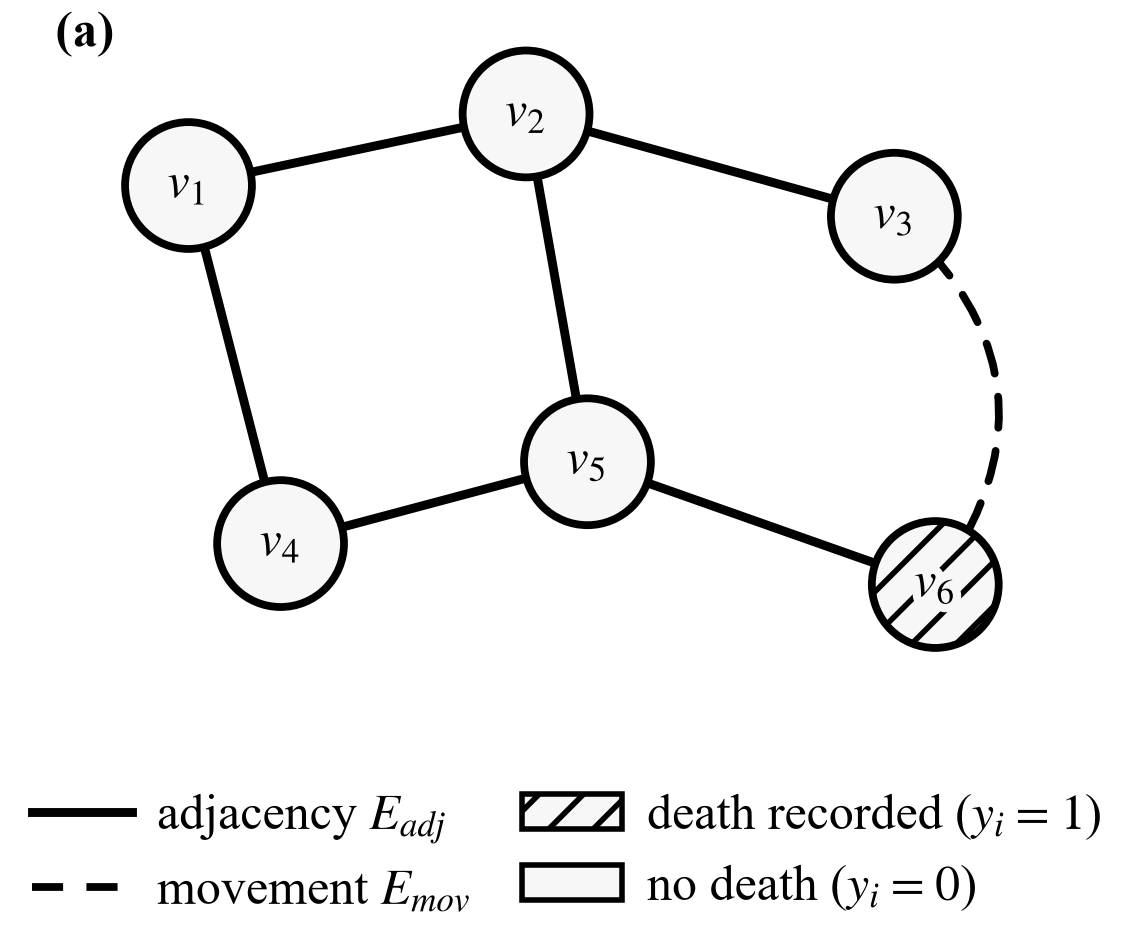
\includegraphics{figures/problem_input.png}
\alt{Graph of six road segments drawn as nodes. Solid lines join physically adjacent segments, and a dashed line joins two segments linked by panther movement. One node is hatched to show a recorded death.}
\caption{Before: the road-segment graph, with recorded deaths marked.}
\label{fig:input}
\end{figure}

\begin{figure}[t]
\centering
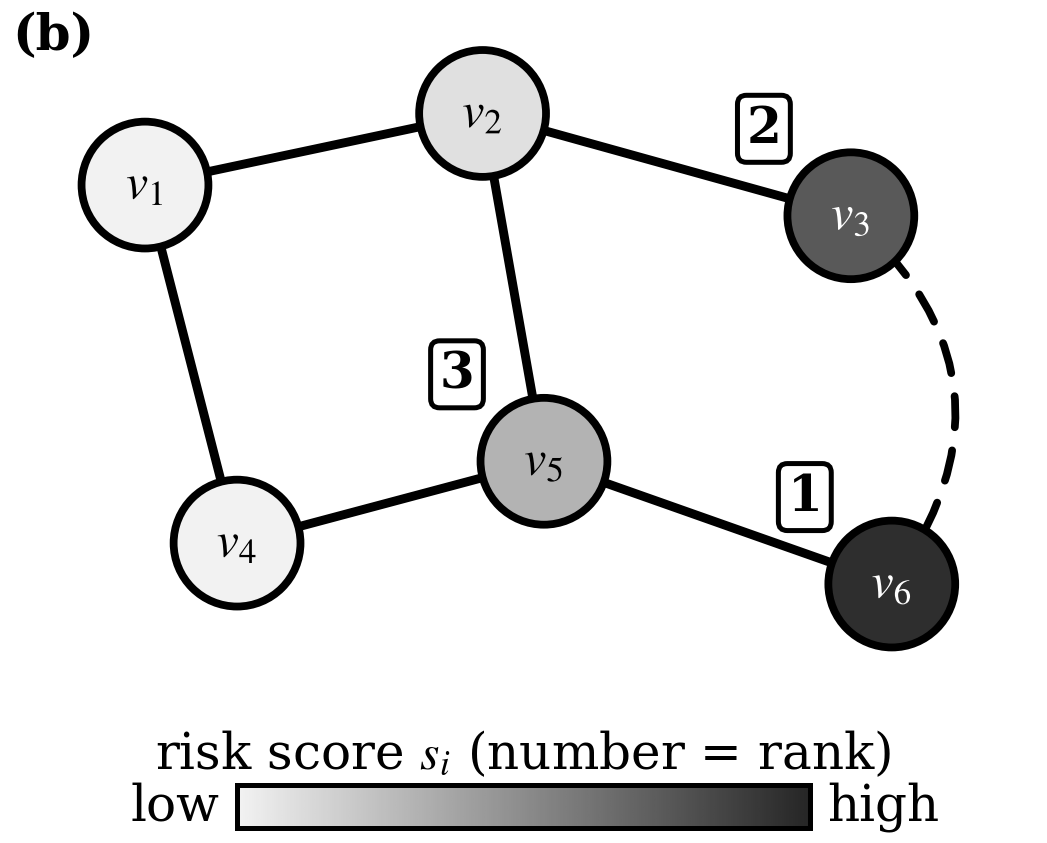
\includegraphics{figures/problem_output.png}
\alt{The same graph with each node shaded by predicted risk from light (low) to dark (high). Three nodes carry rank badges 1, 2, and 3, with rank 1 on the darkest node.}
\caption{After: the same graph, with a risk score and rank for every segment.}
\label{fig:output}
\end{figure}


\section{Methodology}\subsection{Problem Formulation}
We represent the road network as an undirected graph $G = (V, E)$ whose nodes $V = \{v_1, \dots, v_N\}$ are road segments (Figure~\ref{fig:input}). Each segment has a feature vector $\mathbf{x}_i \in \mathbb{R}^d$ and a binary label $y_i \in \{0, 1\}$ (Eq.~\ref{eq:label}) that marks whether a vehicular death was recorded within buffer distance $b$ of it. The edges $E = E_{\mathrm{adj}} \cup E_{\mathrm{mov}}$ join physically adjacent segments and segments linked by panther movement. Given $G$ and $X = [\mathbf{x}_1, \dots, \mathbf{x}_N]^\top$, the task is to learn a function that assigns each segment a risk score $s_i$ so that the highest-ranked segments are the most likely positives (Figure~\ref{fig:output}).

\subsection{Road Segment Graph}

\textbf{Nodes:} Road routes are split at every point where two routes meet or
cross, so each node is a stretch of road between intersections. Each segment
inherits the FDOT road status of its nearest source route. Road segments were
chosen over grid cells because a segment maps directly to the unit a wildlife
agency or transportation planner would act on when siting crossings or
fencing.

\textbf{Adjacency edges:} $(v_i, v_j) \in E_{\mathrm{adj}}$ if the two
segments share an endpoint. Because every intersection is treated as a
junction, overpasses and underpasses are not distinguished.

\textbf{Movement steps:} For each panther, telemetry fixes are sorted by date
and each pair of consecutive fixes is joined by a straight line, called a
movement step, provided the fixes are at most $\Delta_{\max}$ days apart and
at different locations. A straight line is an approximation and not
necessarily the path the panther walked; more sophisticated movement models
exist but add scope beyond this project. A step that intersects a segment is
recorded as a candidate crossing of that segment, and the crossing frequency
$c_i$ of $v_i$ is the number of steps intersecting it.

\textbf{Movement edges:} Let $S(\tau)$ be the set of segments crossed by step
$\tau$. For every step with $2 \le |S(\tau)| \le M$, each pair of segments in
$S(\tau)$ gains one unit of weight, so $w_{ij}$ counts the steps shared by
$v_i$ and $v_j$. We define
$E_{\mathrm{mov}} = \{(v_i, v_j) : w_{ij} \ge w_{\min}\}$, with
$\Delta_{\max} = 30$ days, $M = 6$, and $w_{\min} = 2$. Movement edges link
segments that share panther traffic even when they are not physically
connected. Figure~\ref{fig:step} illustrates how steps accumulate into
movement edges.

\begin{table}[t]
\centering
\small
\begin{tabular}{lr}
\hline
\textbf{Feature} & \textbf{Columns} \\
\hline
Crossing frequency & 1 \\
Fixes within 500~m and 2~km & 2 \\
Panthers within 2~km & 1 \\
Distance to nearest fix & 1 \\
Segment length & 1 \\
Road status (one indicator per code) & 7 \\
\hline
\textbf{Total ($d$)} & \textbf{13} \\
\hline
\end{tabular}
\caption{Node features by number of columns.}
\label{tab:features}
\end{table}

\begin{figure}[t]
\centering
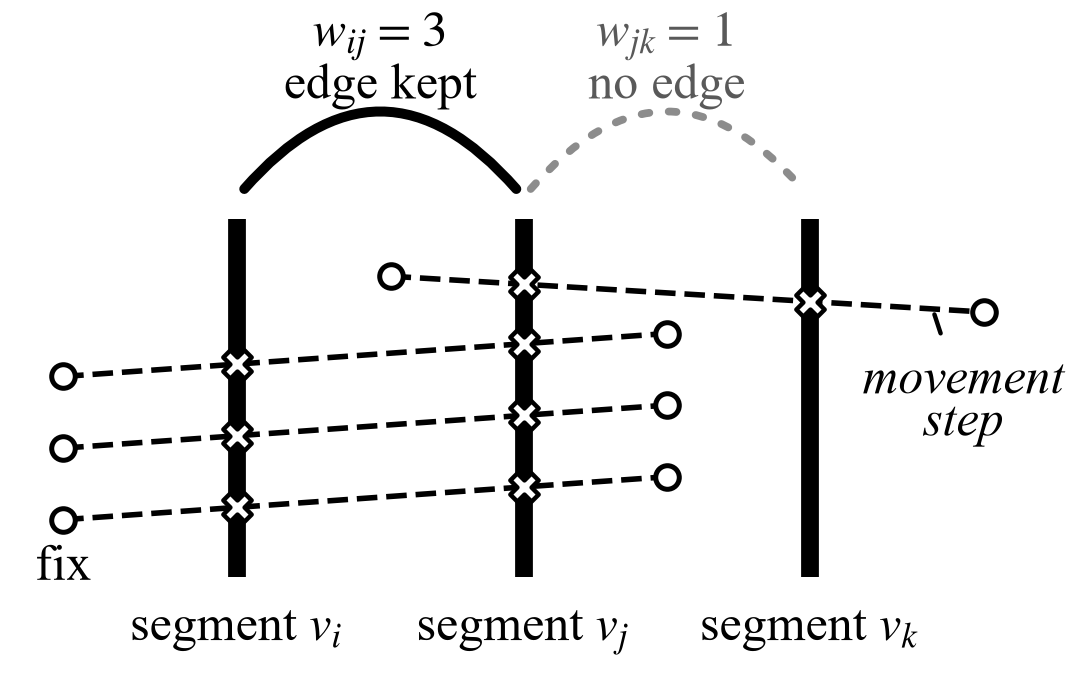
\includegraphics{figures/movement_edges.png}
\alt{Three road segments crossed by dashed lines between telemetry fixes. Three lines cross the first two segments, which are joined by a solid arc labeled w equals 3, edge kept. One line crosses the second and third segments, which are joined by a faint dotted arc labeled w equals 1, no edge. An edge is kept if its weight is at least 2.}
\caption{Weights count the steps shared by two segments; only pairs with $w_{ij} \ge w_{\min}$ become movement edges.}
\label{fig:step}
\end{figure}

\subsection{Node Features and Labels}
Each segment has $d = 13$ features (Table~\ref{tab:features}). Five are
derived from telemetry: the crossing frequency $c_i$, the number of fixes
within 500~m and within 2~km of the segment, the number of distinct panthers
with a fix within 2~km, and the distance from the segment to the nearest fix.
The remaining eight are the segment length in meters and a one-hot encoding of
the seven FDOT road status codes. Speed limit and traffic volume are not attributes of the FDOT layer used here and are left to future
work. A segment is labeled positive if a recorded vehicular death $m_k$ lies within
buffer distance $b$ of it:
\begin{equation}
  y_i = \mathbf{1}\!\left[\min_k \operatorname{dist}(v_i, m_k) \le b\right],
  \label{eq:label}
\end{equation}
where $\operatorname{dist}$ is the shortest distance in meters between the
segment and the death location, and $\mathbf{1}[\cdot]$ is 1 if the condition
holds and 0 otherwise. We report main results at $b = 100$\,m and test
$b = 250$ and $500$\,m as a sensitivity check. Twelve of the 399 deaths lie
more than 500\,m from any segment and therefore label no segment at any
buffer.
\subsection{Graph Model}
We use GraphSAGE~\cite{hamilton2017inductive} with a separate mean
aggregation for each edge type, summed at every layer:
\begin{align}
  \bar{\mathbf{h}}_{i,\mathrm{adj}}^{(\ell)} &= \mathrm{MEAN}\{\mathbf{h}_j^{(\ell-1)} : v_j \in \mathcal{N}_{\mathrm{adj}}(v_i)\}, \nonumber \\
  \bar{\mathbf{h}}_{i,\mathrm{mov}}^{(\ell)} &= \mathrm{MEAN}\{\mathbf{h}_j^{(\ell-1)} : v_j \in \mathcal{N}_{\mathrm{mov}}(v_i)\}, \nonumber \\
  \mathbf{h}_i^{(\ell)} &= \sigma\big(W_{\mathrm{self}}^{(\ell)} \mathbf{h}_i^{(\ell-1)}
    + W_{\mathrm{adj}}^{(\ell)} \bar{\mathbf{h}}_{i,\mathrm{adj}}^{(\ell)} \nonumber \\
  &\qquad + W_{\mathrm{mov}}^{(\ell)} \bar{\mathbf{h}}_{i,\mathrm{mov}}^{(\ell)}\big),
  \label{eq:sage}
\end{align}
where $\mathbf{h}_i^{(0)} = \mathbf{x}_i$, $\mathcal{N}_{\mathrm{adj}}(v_i)$
and $\mathcal{N}_{\mathrm{mov}}(v_i)$ are the neighbors of $v_i$ under
$E_{\mathrm{adj}}$ and $E_{\mathrm{mov}}$, the $W^{(\ell)}$ are learned weight
matrices, $\sigma$ is the rectified linear unit (ReLU), $\sigma(x)=\max(0,x)$, for $\ell = 1$ and the identity for $\ell = 2$, and the mean over an empty
neighborhood is the zero vector. Movement edges are unweighted, and the 69
pairs that are both adjacent and movement-linked appear in both
neighborhoods.

The first layer maps the 13 features to 16 hidden units with ReLU activation;
the second maps these to a single output $z_i = h_i^{(2)}$, and the risk score is
$s_i = 1/(1 + e^{-z_i})$. Dropout with rate 0.5 is applied to the input of
each layer during training.

Features are standardized using the mean and standard deviation of the
training-fold segments, recomputed for each fold. All segments take part in
message passing, but the loss is computed only on training-fold segments;
a test segment may aggregate features from training-fold neighbors across a
block boundary, but test-fold labels are never used. The loss is binary
cross-entropy with the positive class weighted by the ratio of negative to
positive training segments. Training is full-batch with the Adam optimizer \cite{Kingma2015} (adaptive moment estimation) for a fixed 400 epochs at a learning rate of 0.01, following the cross-validation setup of Kipf and Welling~\shortcite{kipf2017semi}, with L2 regularization of $5 \times 10^{-4}$ applied to all weights. To isolate the contribution of movement connectivity, we also train an identical model using only $E_{\mathrm{adj}}$.

\subsubsection{Algorithm Description.} The proposed algorithm for this study applies GraphSAGE for predicting vehicular risk across road segments. This prediction is achieved through incorporating information from neighboring segments. Unlike many Machine Learning models that evaluate segments in an independent manner, GraphSAGE brings a different approach that allows information to propagate through the graph, with the goal of potentially capturing relationships between segments associated with panther movement.
The following steps describe the algorithm's operation:


\begin{enumerate}
    \item \textbf{Input representation:} Each road segment is represented by a 13-dimensional feature vector. In this case, two types of connections are taken into consideration: physical road adjacency and movement-derived connectivity from panther telemetry.

    \item \textbf{Neighborhood aggregation:} For each segment, GraphSAGE computes the mean feature representations of its physically adjacent neighbors and movement-connected neighbors. This calculation is done independently for each segment.

    \item \textbf{Feature transformation:} The aggregated representations are then combined with the segment's own features. This is done through learned weight matrices. The first layer then produces 16-dimensional hidden representations using ReLU activation method.

    \item \textbf{Risk prediction:} At this stage, a second aggregation layer produces a single output for each of the segments. A sigmoid function then transforms this output into a predicted mortality-risk score, which varies between 0 and 1.

    \item \textbf{Model optimization:} The model is trained using class-weighted binary cross-entropy to account for the low proportion of positive segments, which is 6.2\% with the 100 m buffer. Training uses Adam optimization with dropout and L2 regularization. This is done aiming to reduce overfitting.
\end{enumerate}

\subsubsection{Design Rationale.} GraphSAGE was selected for this study because it can incorporate relationships between road segments that traditional non-graph models would not be able to represent. By separating physical adjacency from movement-derived connectivity, the algorithm provides the ability to learn distinct spatial relationships. The two-layer architecture enables information aggregation across neighborhoods while maintaining relatively low model complexity. Finally, class-weighted training addresses the problem of imbalance between segments with and without recorded vehicular mortality.

% \section{Experiments}
% ~0.75 page
% \begin{itemize}
% \item Dataset(s) with source, size, and splits; (Jeremy)
% \begin{itemize}
% \item dataset stats; (Jeremy)
% \end{itemize}
% \item at least one baseline method; (Jeremy)
% \begin{itemize}
% \item baselines defined; (Jeremy)
% \end{itemize}
% \item evaluation metrics with definitions; (Jeremy)
% \item  train/validation/test protocol; (Jeremy)
% \item reproducibility details. (Jeremy)
% \end{itemize}
\section{Experiments}

\subsection{Datasets \& Exploratory Statistics}
We use three public datasets (Table~\ref{tab:data}). Panther telemetry and mortality records come from the Florida Fish and Wildlife Conservation Commission (FWC) \cite{FWCPantherTelemetry,FWCPantherMortality}; the road network is the FDOT Linear Referencing System (LRS) Routes with Measures layer \cite{FDOTLRS}. All layers are reprojected to a common metric coordinate system (North American Datum 1983 (NAD83), Universal Transverse Mercator (UTM) zone 17N, European Petroleum Survey Group (EPSG) code 26917) so that buffers, distances, and spatial blocks are measured in meters.

\begin{table}[t]
\centering
\small
\begin{tabular}{lrr}
\hline
\textbf{Dataset} & \textbf{Raw} & \textbf{In scope} \\
\hline
Telemetry fixes & 112{,}802 & 63{,}170 \\
Vehicular deaths & 461 & 399 \\
Road routes & 18{,}405 & 765 \\
\hline
\end{tabular}
\caption{Dataset sizes before and after scoping.}
\label{tab:data}
\end{table}

We keep telemetry fixes and vehicular-trauma deaths from 2000 onward, and roads and deaths in Collier, Hendry, Lee, and Glades counties, the study area defined in the Introduction. This leaves 63{,}170 fixes from 219 panthers, 399 vehicular deaths, and 765 road routes (3{,}838~km). Fixes come from aerial very high frequency (VHF) tracking, and 98.8\% were recorded between 07:00 and 17:00, so they are sparse snapshots, not continuous tracks. We start in 2000 because recorded vehicular deaths rise sharply from that year onward, and this cutoff retains 93.5\% of all vehicular deaths (431 of 461) while discarding the sparsely recorded early years. Only 27 of the 399 deaths involve a panther that appears in the telemetry, so we treat the tracked panthers as a sample of population-level movement rather than a record of the animals that died.

Routes are split at every intersection into $N=2{,}631$ road segments (median length 600~m), which are the nodes of the graph. The graph has 5{,}637 physical-adjacency edges and 243 movement-derived edges, 174 of which link segments that are not physically adjacent. A segment is labeled positive if a vehicular death lies within a buffer distance $b$ of it; Table~\ref{tab:labels} gives the number of positive segments at each buffer. Because positives are this rare, a trivial ``no strike'' predictor, which labels every one of the $N$ segments negative, would exceed 90\% accuracy at every buffer (last column of Table~\ref{tab:labels}), so we do not report accuracy.


\begin{table}[t]
\centering
\small
\begin{tabular}{rrrr}
\hline
\textbf{$b$ (m)} & \textbf{Positives} & \textbf{Positive rate} & \textbf{No-strike accuracy} \\
\hline
100 & 163 & 6.2\% & 93.8\% \\
250 & 194 & 7.4\% & 92.6\% \\
500 & 218 & 8.3\% & 91.7\% \\
\hline
\end{tabular}
\caption{Label imbalance by buffer distance $b$.}
\label{tab:labels}
\end{table}

\subsection{Experimental Setup}
\subsubsection{Baselines.} We compare against three baselines. \textbf{Random forest} \cite{Breiman2001} (300 trees, minimum leaf size 3, class-weighted) and \textbf{XGBoost} \cite{Chen2016XGBoost} (300 trees, depth 4, learning rate 0.05, positive-class weight set to the training class ratio) use the same 13 node features as the graph model (Table~\ref{tab:features}) but no graph structure; they are standard tree-based baselines for imbalanced tabular prediction, and random forests have been used for wildlife--vehicle collision risk \cite{pagany2022spatiotemporal}. A \textbf{kernel density} baseline fits a Gaussian kernel density estimate (KDE; bandwidth 2~km) to historical deaths in the training folds and scores each test segment at its midpoint, projecting past strikes onto the road network without using features. To isolate the contribution of movement connectivity, we also train an adjacency-only variant of the graph model that uses the physical-adjacency edges alone, on the same folds.

\subsubsection{Evaluation Metrics.} Let $y_i\in\{0,1\}$ be the label of segment $i$ and $s_i$ a model's risk score. Metrics are computed on each held-out fold and reported as mean $\pm$ standard deviation.
\textbf{AUC-PR}, the primary metric, is the average precision of the ranking by $s_i$; a random scorer scores about the positive rate (0.062 at $b=100$~m).
\textbf{Recall at the top $p$\%}, for $p\in\{5,10\}$, is the fraction of a fold's positive segments that appear among its $p$\% highest-scoring segments, reflecting the share of mortality an agency would capture by treating that fraction of the road network; a random scorer scores $p$\%.
\textbf{Brier score} $\frac{1}{N_f}\sum_i (s_i-y_i)^2$, averaged over the $N_f$ segments of a held-out fold, measures calibration when the risk score $s_i$ is a predicted probability (lower is better); it is undefined for the KDE baseline, whose output is a density.

\subsubsection{Evaluation Protocol.} Random $k$-fold splits would place neighboring, graph-connected segments in both training and test sets. We instead use spatial block cross-validation: segment midpoints are assigned to 15~km square blocks (67 blocks), and whole blocks are assigned to $5$ folds, largest first, to balance fold sizes (Figure~\ref{fig:folds}). A segment belongs to the block containing its midpoint, so long segments can extend into neighboring blocks and segments in different folds can touch at block boundaries. Each fold holds about 526 segments and between 18 and 41 positive segments at $b=100$~m. Each model is trained on four folds and tested on the fifth; all models, including the graph model, use identical folds, and each death is assigned to the fold of its nearest segment so the KDE is fit only on training-fold deaths. Hyperparameters are fixed in advance and not tuned, so no separate validation split is needed; this avoids selecting settings on test folds. Paired per-fold differences are used to check that a model's advantage is consistent rather than driven by one fold.



\begin{figure}[t]
\centering
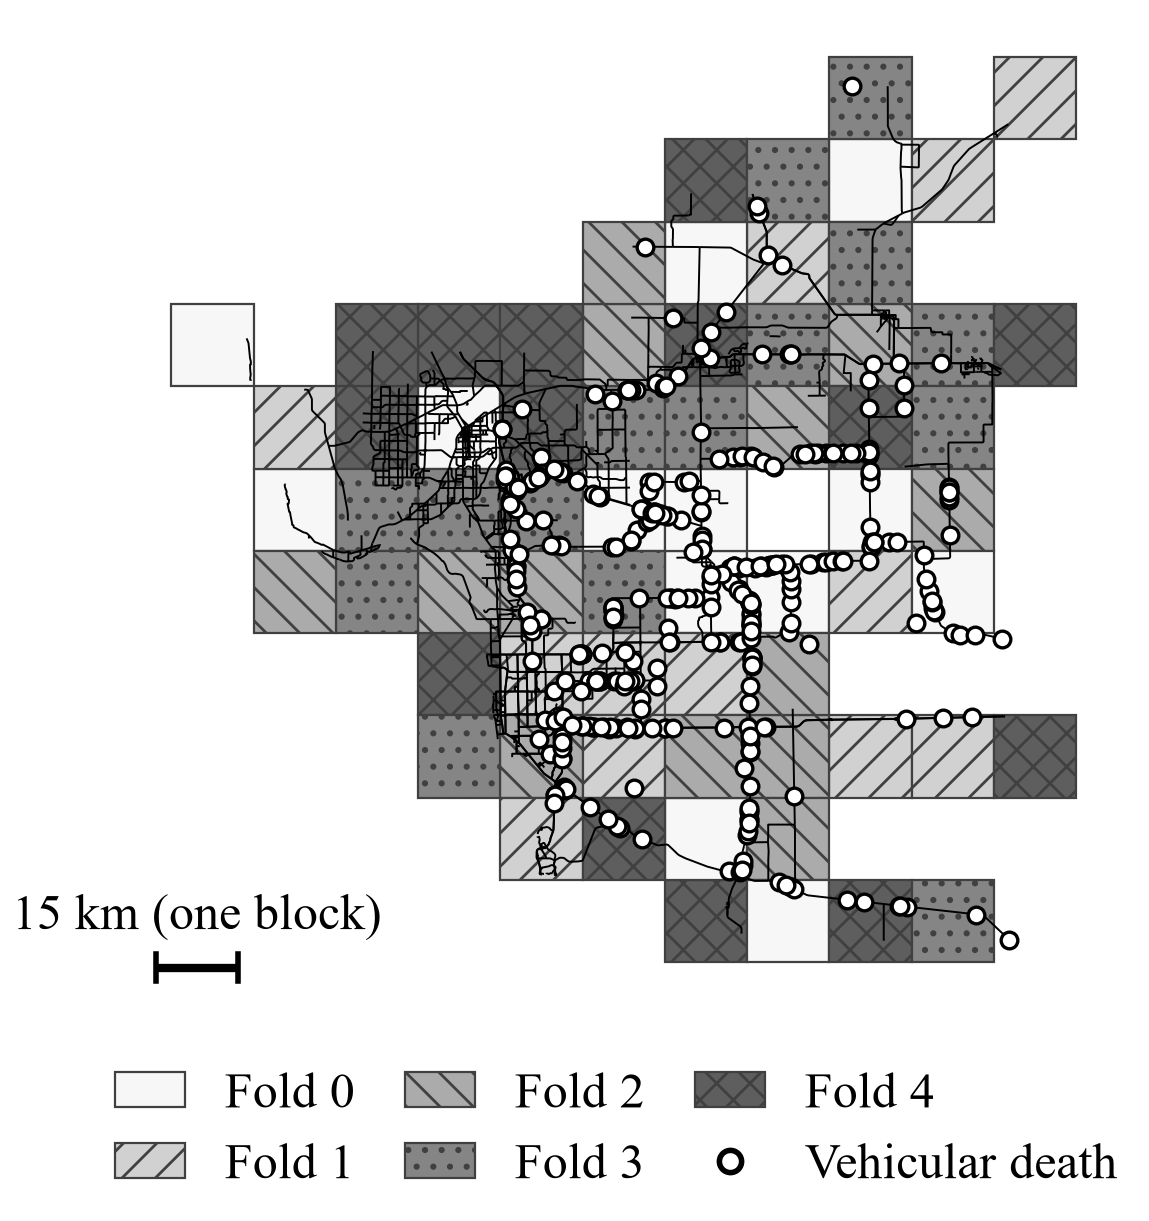
\includegraphics[width=\columnwidth]{figures/study_map_folds.png}
\alt{Map of the four-county study area. Road segments are drawn as black lines over 15 kilometer square blocks, each shaded and patterned by one of five cross-validation folds. Open circles mark vehicular deaths, which concentrate along a few major roads in the center and west.}
\caption{Road segments, vehicular deaths, and the five spatial cross-validation folds.}
\label{fig:folds}
\end{figure}

\subsubsection{Reproducibility.} All experiments are run from a single Jupyter notebook that reads the three datasets and fixes every parameter in one configuration cell: movement-step gap limit (30 days), minimum movement-edge weight (2), maximum segments per step (6), label buffers (100/250/500~m; 100~m for the main results), block size (15~km), and random seed (42). Software versions are Python with scikit-learn 1.9.0, XGBoost 3.4.1, GeoPandas 1.1.4, Shapely 2.1.2, and NetworkX 3.6.1. The notebook, datasets, and a dataset README are provided with the submission.


% Downs2014, Grace2017
% https://www.floridapantherprotection.com/pdf/Downs%20et%20al%202013%20Strategically%20Locating%20Cross%20Structures.pdf is a pretty good target for talking about crossing placment
% https://journals.sagepub.com/doi/10.3141/2270-05
% https://floridawildlifefederation.org/wp-content/uploads/2026/06/Design-Guide-For-Wildlife-Crossings-Version-1.1-06_24_26.pdf

\bibliographystyle{flairs}
\bibliography{references}

\section{AI Usage Statement}
During the preparation of this work, the authors used Anthropic's Claude to assist in rewording text, correcting grammatical errors, drafting tables, and drafting and debugging Python code for the experiment notebook, including dataset statistics and figure generation. The authors reviewed and verified all code output, edited the text, and take full responsibility for the content of this publication. The research question, experimental design, analysis, and conclusions are the authors' own.

\section{Team Contribution Statement}
\textbf{George Alenchery: } Introduction; Methodology (problem formulation, road-segment
graph construction, node features and labels, graph model) \\
\textbf{Jeremy Martin: } Experiments (datasets and exploratory statistics, baseline methods, evaluation metrics, evaluation protocol, reproducibility); Jupyter notebook implementation of data preparation, features, labels, spatial cross-validation, and baseline models \\
\textbf{Marcelo Amorim: } Introduction (rephrasing on Motivation and Related Works); Methodology (Algorithm Description, Design Rationale)\\

\end{document}
